% SciPy: Posters are commonly 36 or 42 inches tall and can be 72 inches wide.
\documentclass[a0paper,fleqn]{betterposter}
\usepackage{bm}
\graphicspath{{figures/}}

%%%% Uncomment the following commands to customise the format

%% Setting the width of columns
% Left column
\setlength{\leftbarwidth}{0.27\paperwidth}
% Right column
\setlength{\rightbarwidth}{0.27\paperwidth}

%% Setting the column margins
% Horizontal margin
%\setlength{\columnmarginvertical}{0.05\paperheight}
% Vertical margin
%\setlength{\columnmarginhorizontal}{0.05\paperheight}
% Horizontal margin for the main column
%\setlength{\maincolumnmarginvertical}{0.15\paperheight}
% Vertical margin for the main column
%\setlength{\maincolumnmarginhorizontal}{0.15\paperheight}

% %% Changing font sizes
% % \fontsize{font size to use}{baselineskip to use}
% % Text font
% \renewcommand{\fontsizestandard}{\fontsize{28}{35} \selectfont}
% % \renewcommand{\fontsizestandard}{\fontsize{26}{32.5} \selectfont}
% % \renewcommand{\fontsizestandard}{\fontsize{26}{35} \selectfont}
% % Main column font
% %\renewcommand{\fontsizemain}{\fontsize{28}{35} \selectfont}
% \renewcommand{\fontsizemain}{\fontsize{148}{280} \selectfont}
% % Title font
% %\renewcommand{\fontsizetitle}{\fontsize{28}{35} \selectfont}
% % Author font
% % \renewcommand{\fontsizeauthor}{\fontsize{28}{35} \selectfont}
% % \renewcommand{\fontsizeauthor}{\fontsize{26}{32.5} \selectfont}
% \renewcommand{\fontsizeauthor}{\fontsize{26}{35} \selectfont}
% \newcommand{\fontsizeinstitution}{\fontsize{16}{25} \selectfont}
% % Section font
% %\renewcommand{\fontsizesection}{\fontsize{28}{35} \selectfont}
% \renewcommand{\fontsizesection}{\fontsize{61.00}{87.00} \selectfont}

% \renewcommand{\fontsizestandard}{\fontsize{41.00}{64} \selectfont}
\renewcommand{\fontsizestandard}{\fontsize{32}{46} \selectfont}
\renewcommand{\fontsizemain}{\fontsize{148.00}{280.00} \selectfont}
\renewcommand{\fontsizetitle}{\fontsize{101.50}{152.00} \selectfont}
\renewcommand{\fontsizeauthor}{\fontsize{33.55}{47.3} \selectfont}
\renewcommand{\fontsizesection}{\fontsize{61.00}{86.00} \selectfont}
\renewcommand{\fontsizesubsection}{\fontsize{48.00}{57.00} \selectfont}
% \newcommand{\fontsizeinstitution}{\fontsize{16}{25} \selectfont}
\newcommand{\fontsizeinstitution}{\fontsize{20}{25} \selectfont}

%% Changing font sizes for a specific text segment
% Place the text inside brackets:
% {\fontsize{28}{35} \selectfont Your text goes here}

%% Changing colours
% Background of side columns
%\renewcommand{\columnbackgroundcolor}{black}
% Font of side columns
%\renewcommand{\columnfontcolor}{gray}
% Background of main column
%\renewcommand{\maincolumnbackgroundcolor}{empirical}
%\renewcommand{\maincolumnbackgroundcolor}{theory}
%\renewcommand{\maincolumnbackgroundcolor}{methods}
%\renewcommand{\maincolumnbackgroundcolor}{intervention}
% Font of main column
%\renewcommand{\maincolumnfontcolor}{gray}

% Disable hyphenation
\hyphenpenalty=10000
\exhyphenpenalty=10000

\begin{document}
\betterposter{
 % MAIN COLUMN

 \maincolumn{
  % Main space

  \textbf{pyhf} is a \textbf{pure Python} statistical fitting library that uses \textbf{tensors} and \textbf{autograd} to speed up physics analysis at the LHC
 }{
  % Bottom space

  % QR code
  \qrcode{qr_code.pdf}{smartphoneWhite}{
   \textbf{Take a picture} to
   \\visit the pyhf website
  }
 }

}{
 % LEFT COLUMN

 \title{pyhf}
 \vspace{-1em}
 \textbf{pure Python implementation of HistFactory}

 \author{{\underline{Matthew Feickert}$^{1}$}, {Lukas Heinrich$^{2}$}, {Giordon Stark$^{3}$}, {Kyle Cranmer$^{4}$}}
 \institution{1 Southern Methodist University, 2 CERN, 3 University of California Santa Cruz, 4 New York University}
 %
 \section{HistFactory}
 One of the most widely used statistical models in \textbf{high energy physics} for binned measurements and searches

 \begin{center}
  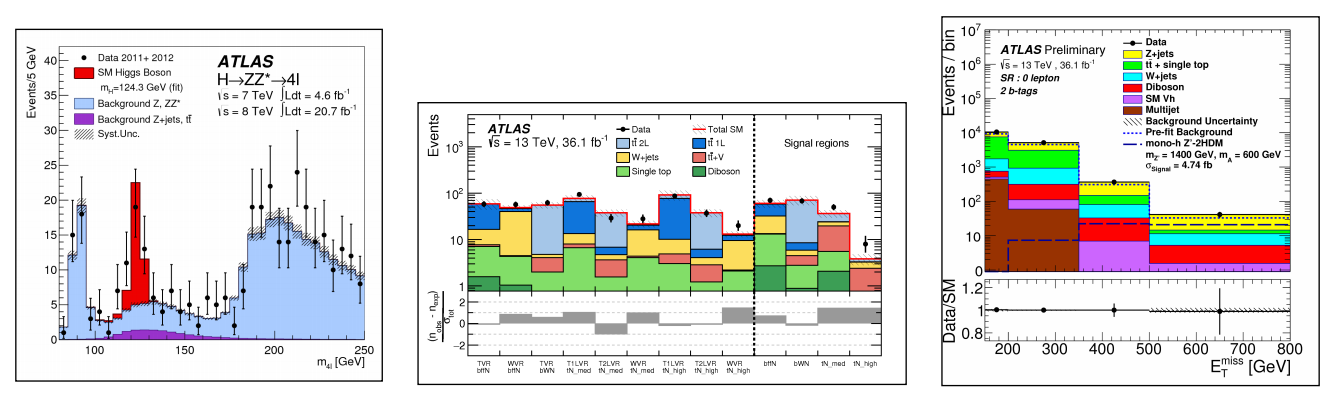
\includegraphics[width=\textwidth]{HistFactory_result_examples.png}
 \end{center}

 \textbf{Declarative binned likelihoods}
 \vspace{1em}
 \[
  f(\bm{n}, \bm{a} \,|\,\bm{\phi},\bm{\chi}) = \underbrace{\color{blue}{\prod_{c\in\mathrm{\,channels}} \prod_{b \in \mathrm{\,bins}_c}\textrm{Pois}\left(n_{cb} \,\middle|\, \nu_{cb}\left(\bm{\eta},\bm{\chi}\right)\right)}}_{\substack{\text{Simultaneous measurement}\\%
    \text{of multiple channels}}} \underbrace{\color{red}{\prod_{\chi \in \bm{\chi}} c_{\chi}(a_{\chi} |\, \chi)}}_{\substack{\text{constraint terms}\\%
    \text{for }\text{``auxiliary measurements''}}}
 \]
 %}
 \vspace{1em}

 \textcolor{blue}{Primary Measurement}:
 \begin{itemize}
  \item Multiple disjoint ``channels'' (e.g.\!\!\!\! event observables) each with multiple bins of data
  \item Example parameter of interest: strength of physics signal, $\mu$
 \end{itemize}
 \textcolor{red}{Auxiliary Measurements}:
 \begin{itemize}
  \item Nuisance parameters (e.g.\!\!\!\! in-situ measurements of background samples)
  \item Systematic uncertainties (e.g. normalization, shape, luminosity)
 \end{itemize}

 \vfill
 \section{Performance}
 Efficient use of tensor computation makes pyhf fast
 \begin{center}
  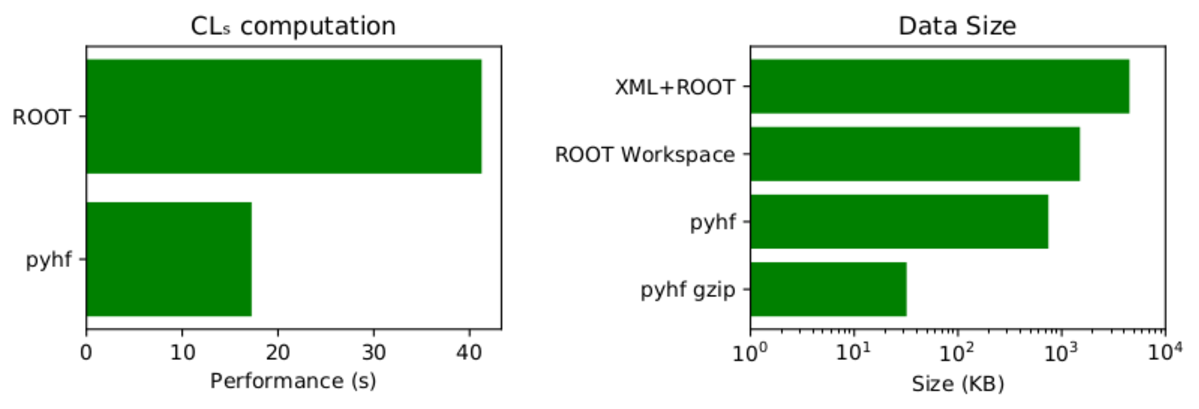
\includegraphics[width=\textwidth]{performance_only.pdf}
 \end{center}
 Competitive with traditional \texttt{C++} implementation --- often faster
 % \vspace{-1em}
 %
 \vfill
 \subsection{Hardware Acceleration}
 For ML-library tensor backends the computational graph can be transparently placed on hardware accelerators: \textbf{GPUs} and \textbf{TPUs} for order of magnitude speed-up in computation
 \begin{center}
  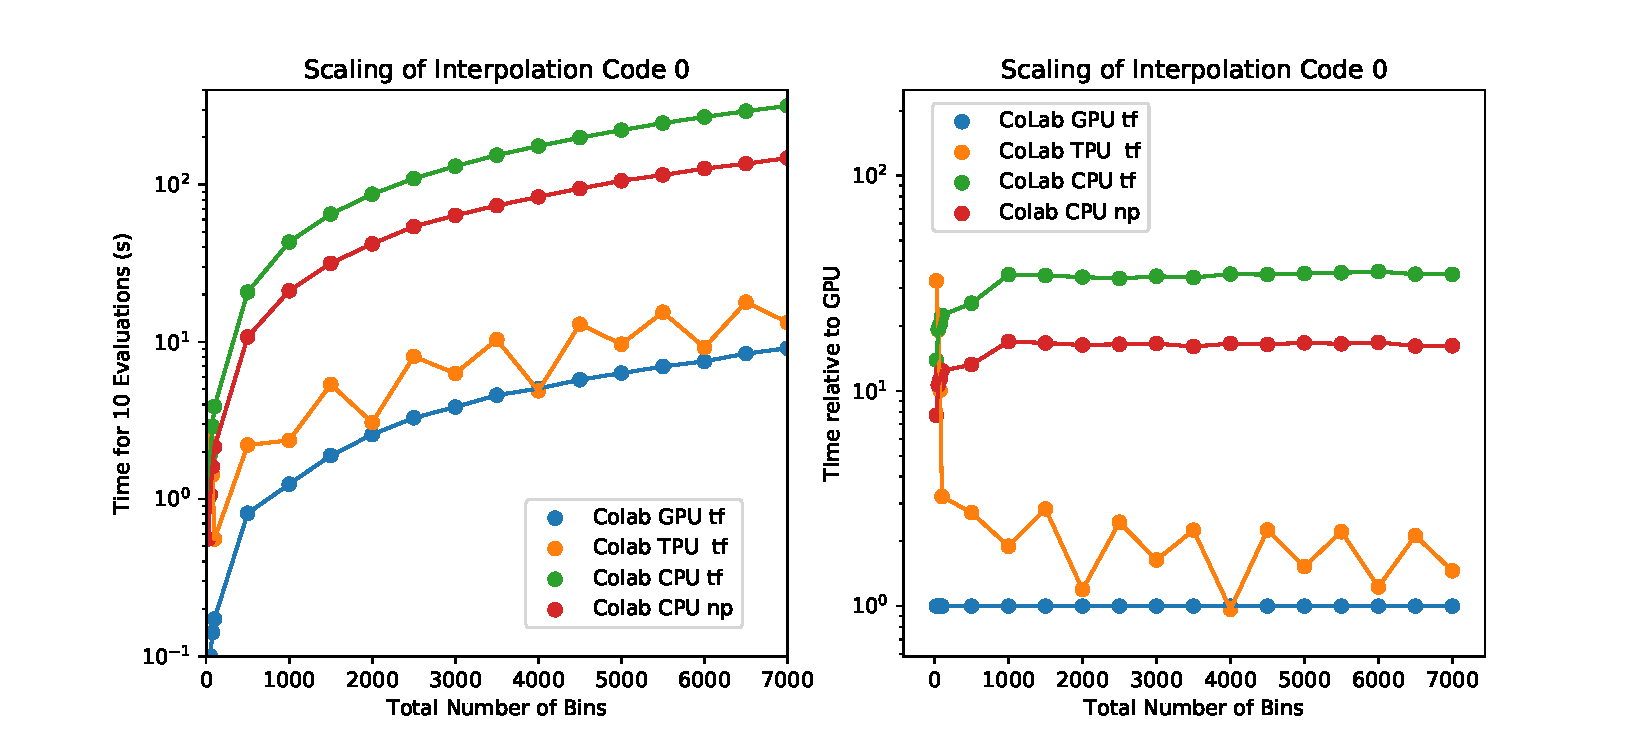
\includegraphics[width=\textwidth]{scaling_hardware.pdf}
 \end{center}
}{
 % RIGHT COLUMN

 \subsection{Implementation}
 \begin{center}
  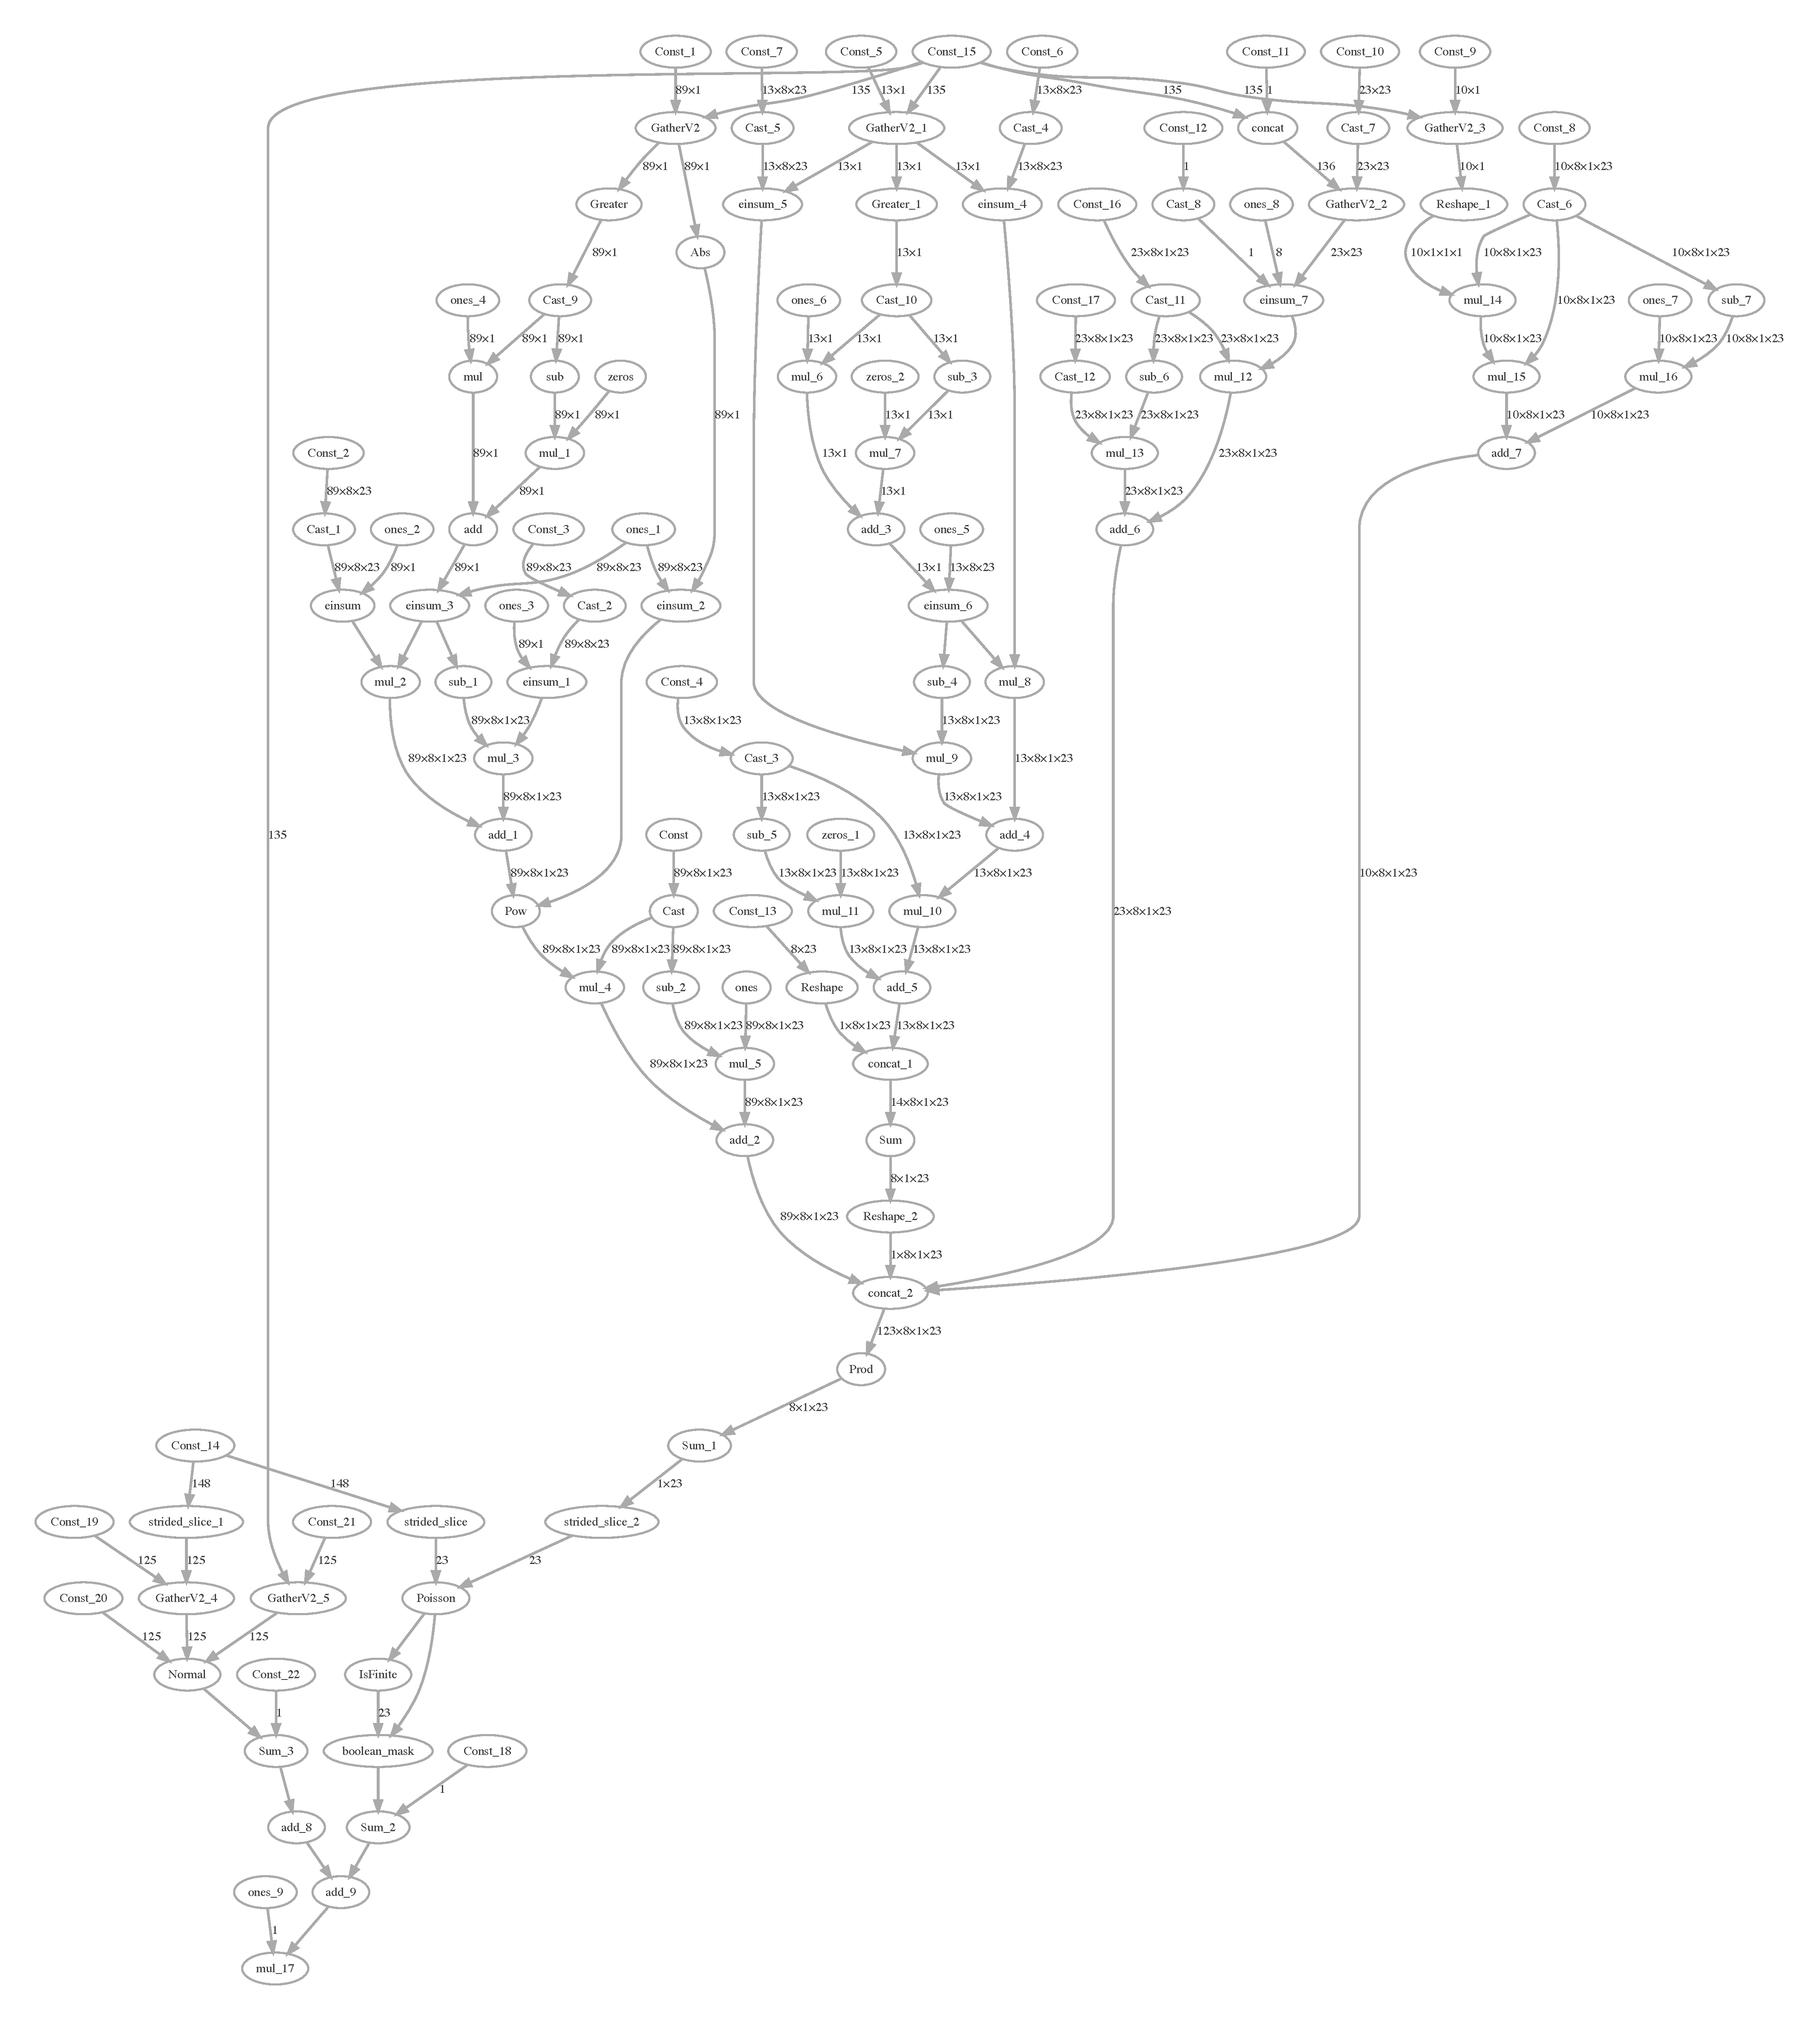
\includegraphics[width=0.9\textwidth]{computational_graph3.pdf}
 \end{center}
 The computational graph of multidimensional array operations for likelihood function of a physics analysis defined through HistFactory

 %
 \vspace{0.5em}
 %
 \begin{minipage}{0.33\textwidth}
  \begin{center}
   
\includegraphics[width=\textwidth]{NumPy_logo.pdf}
  \end{center}
 \end{minipage}%
 \quad
 \begin{minipage}{0.33\textwidth}
  \begin{center}
   
\includegraphics[width=\textwidth]{TensorFlow_logo.pdf}
  \end{center}
 \end{minipage}%
 \quad
 \begin{minipage}{0.33\textwidth}
  \begin{center}
   
\includegraphics[width=0.85\textwidth]{Pytorch_logo.pdf}
  \end{center}
 \end{minipage}%
 %
 \vspace{0.5em}
 %

 Use of array (``tensor'') operations through a common API layer around high performance tensor libraries

 \vspace{-1em}
 \subsection{JSON Specification}
 The full likelihood can be expressed as a \textbf{single JSON document}\\
 Archive friendly for analysis presentation
 \vspace{0.5em}
 \begin{center}
  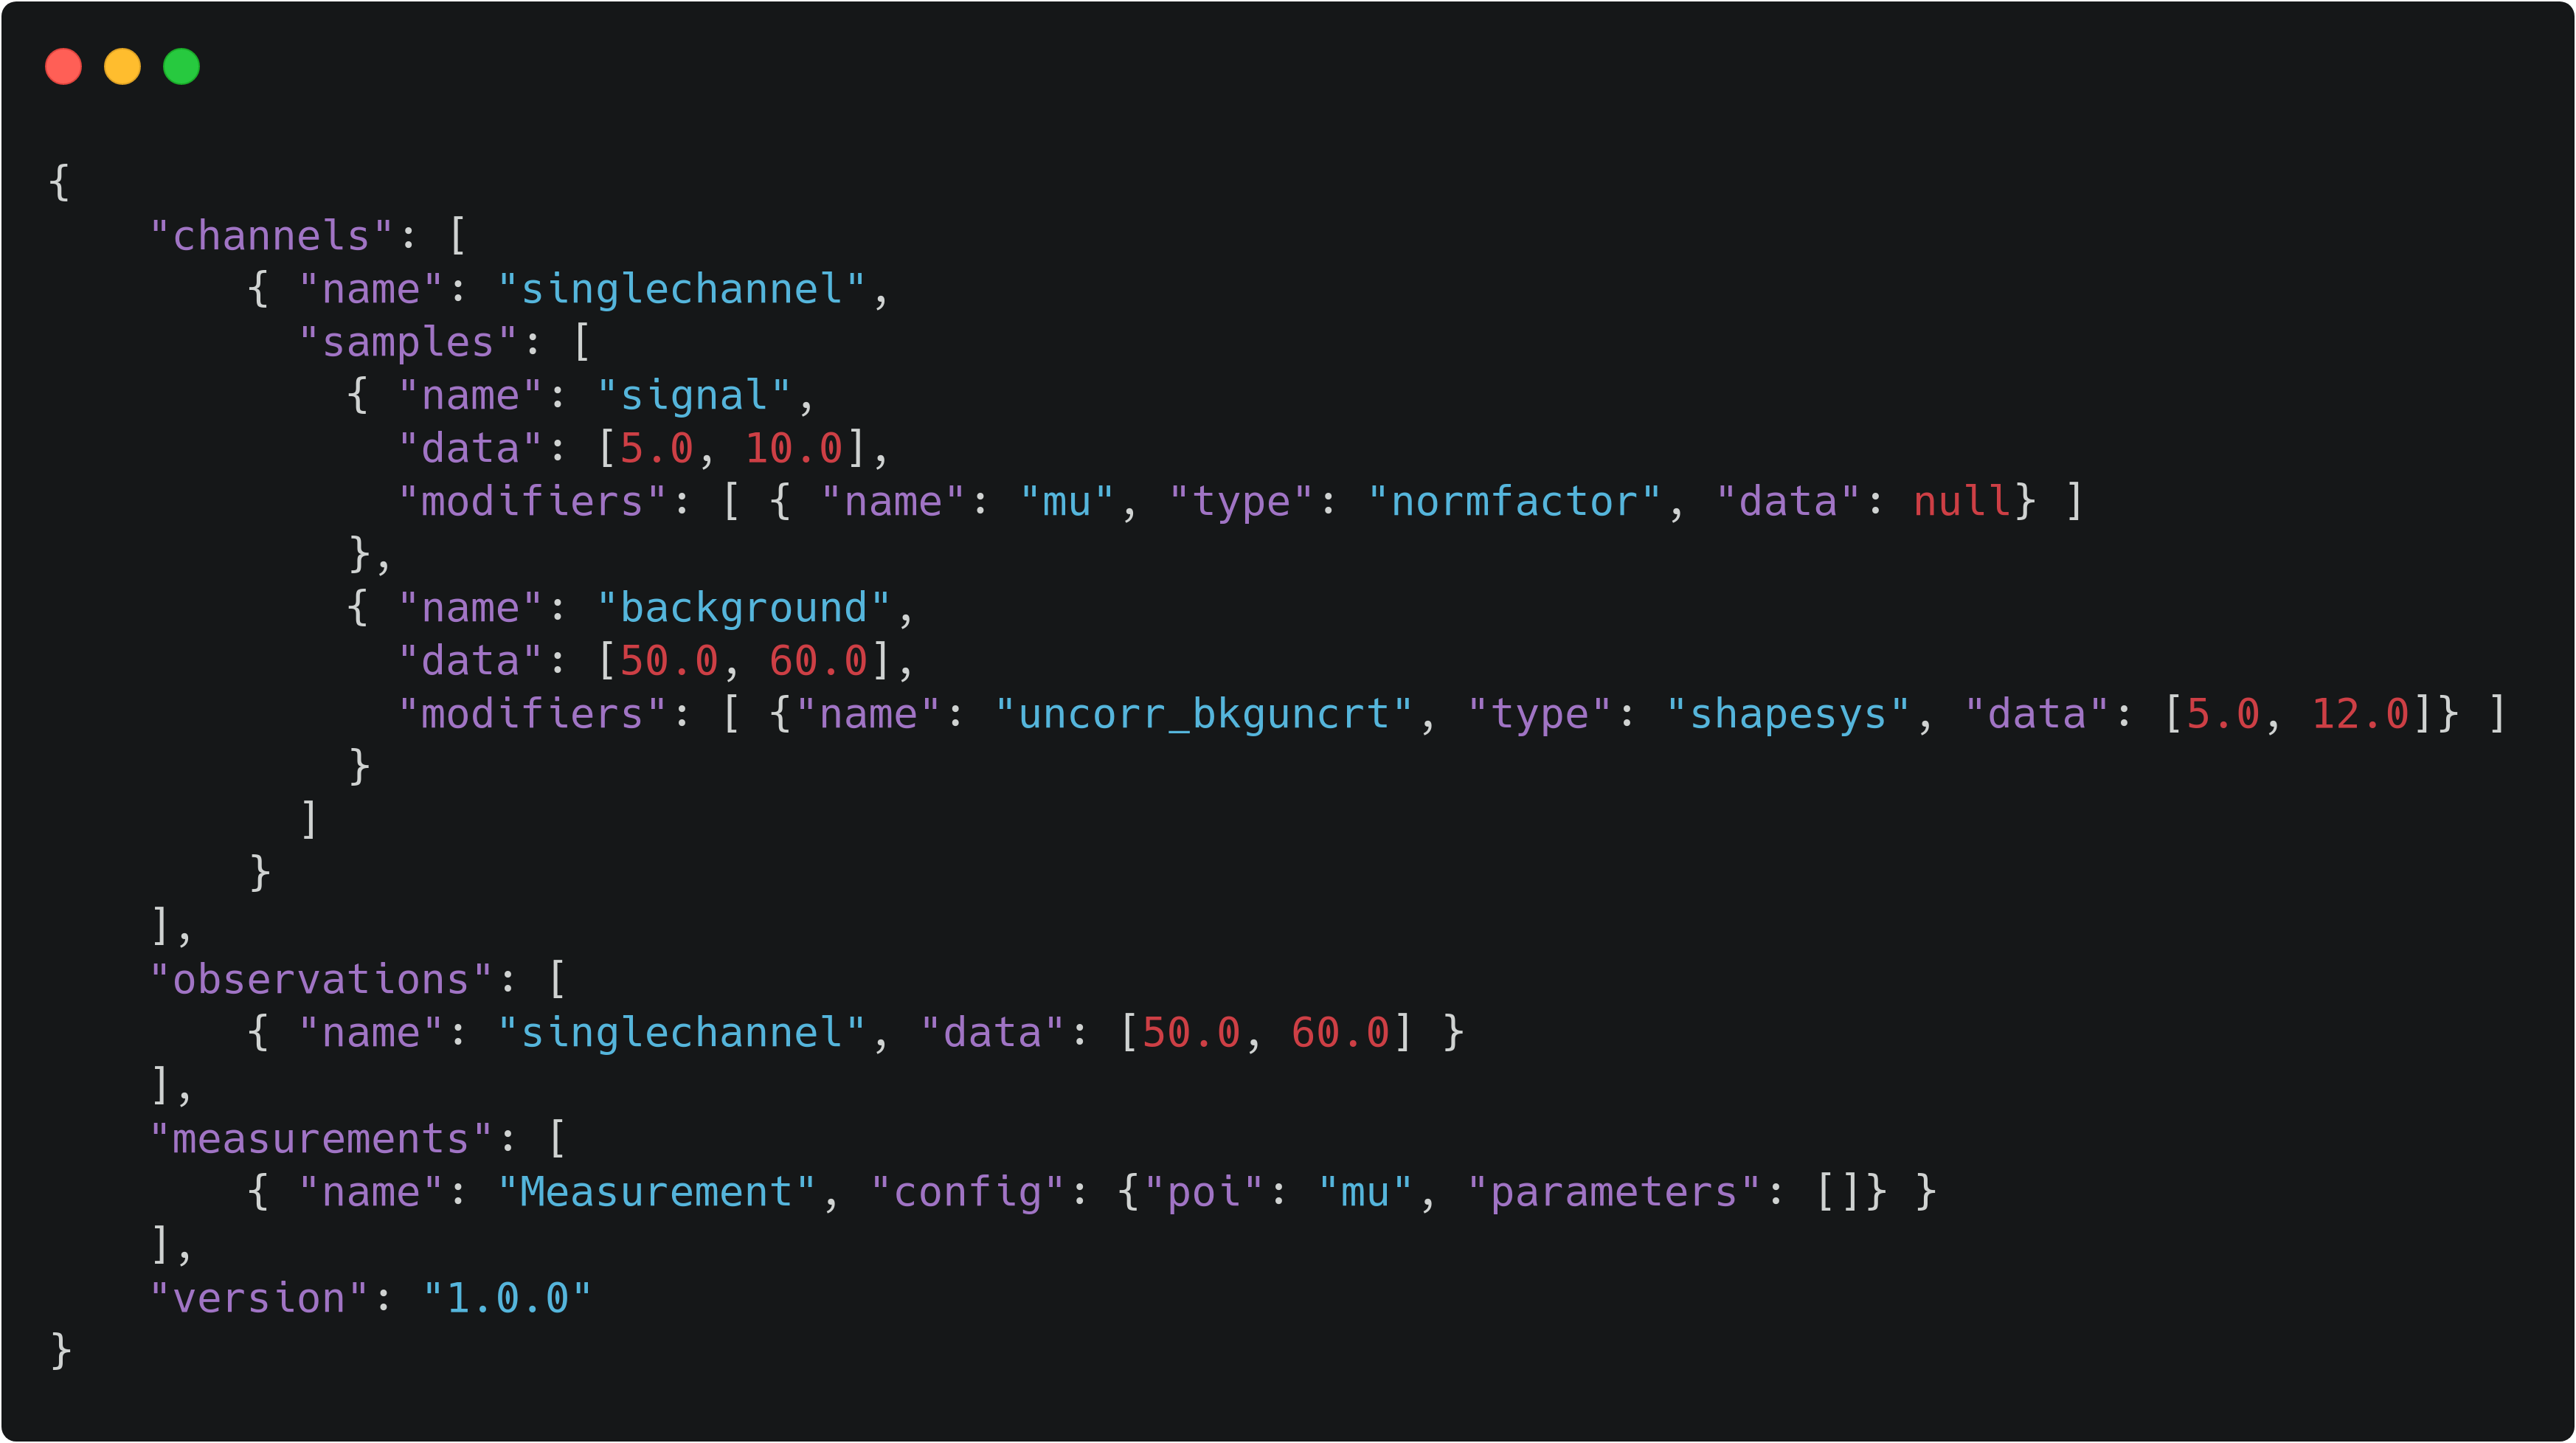
\includegraphics[width=0.9\textwidth]{carbon_JSON_spec.png}
 \end{center}
 \vspace{-1em}
 \begin{center}
  {\fontsizeinstitution\textbf{Example:} 2 binned single channel with 2 samples with 1 parameter of interest and 1 nuisance parameter}
 \end{center}
 \begin{center}
  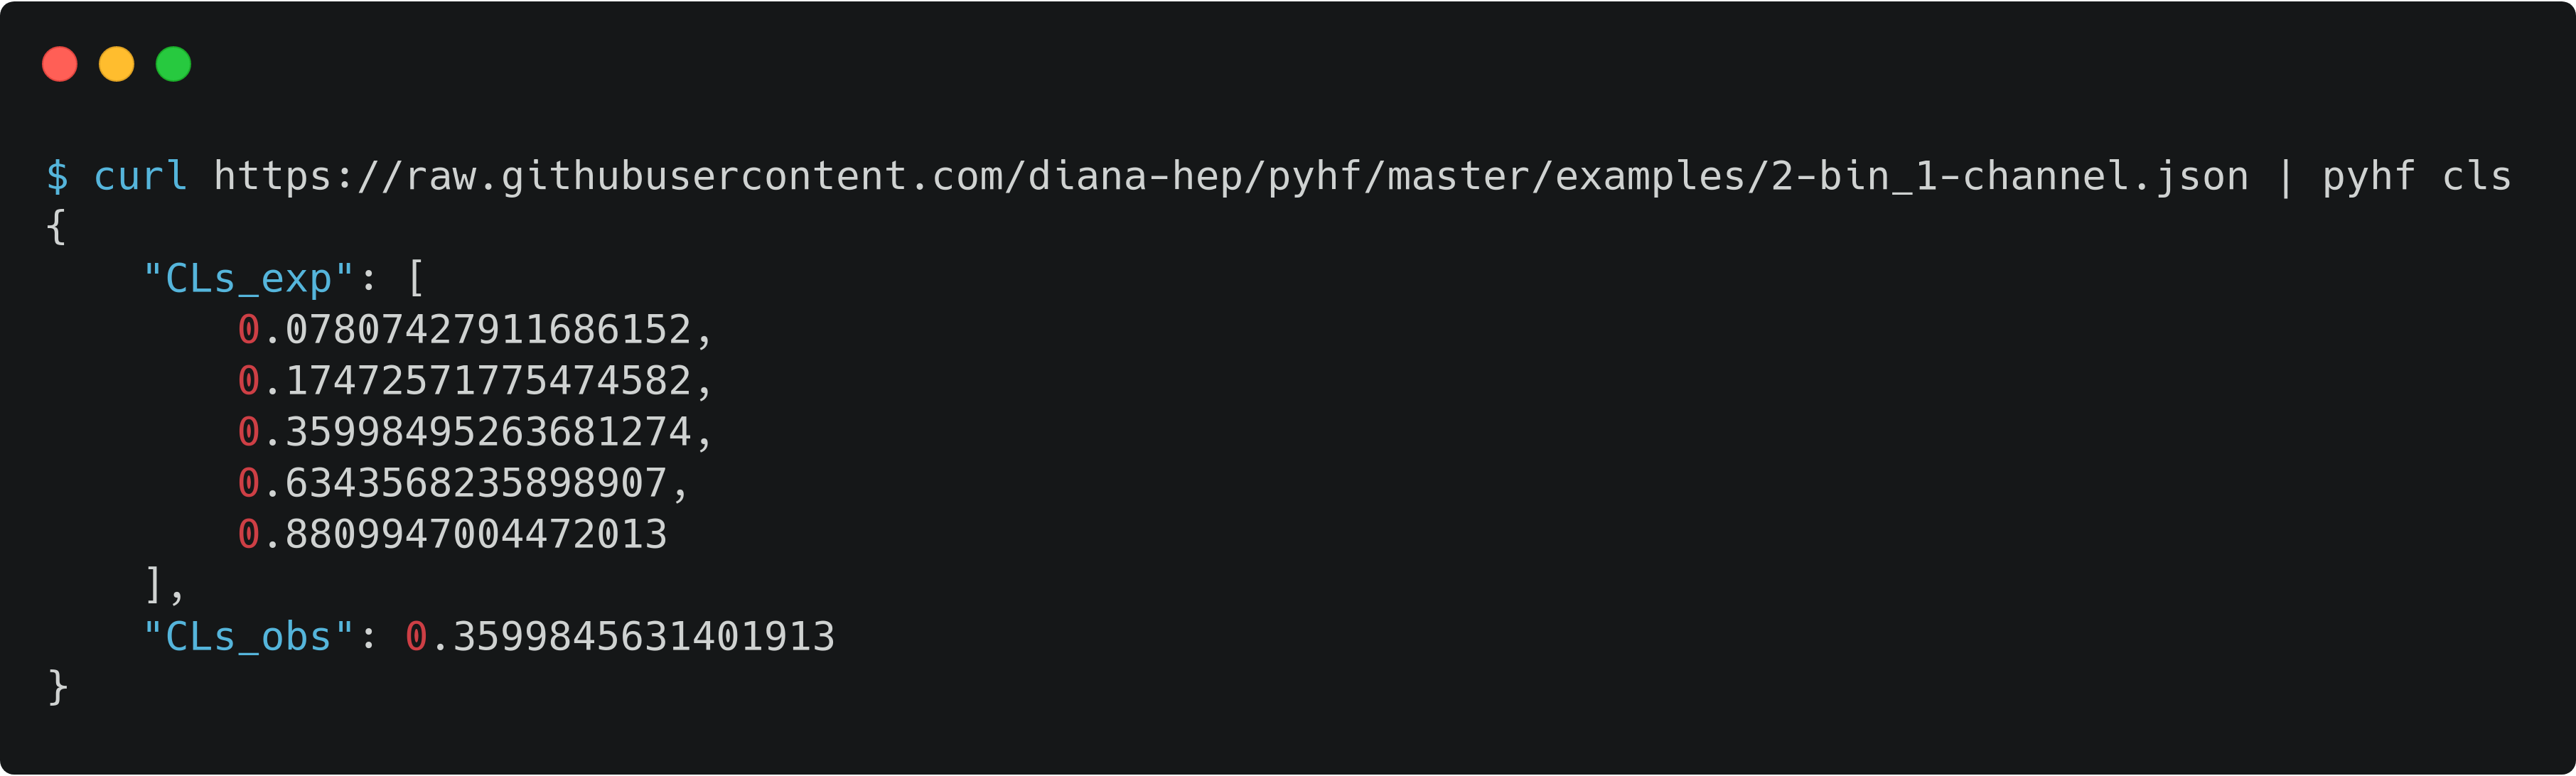
\includegraphics[width=0.9\textwidth]{carbon_pyhf_CLs.png}
 \end{center}

 \vspace{1em}
 \vfill
 \begin{minipage}{0.58\textwidth}
  \begin{center}
   
\includegraphics[width=\textwidth]{IRIS-HEP_logo}
  \end{center}
 \end{minipage}%
 \quad
 \begin{minipage}{0.38\textwidth}
  \begin{center}
   
\includegraphics[width=\textwidth]{pyhf_PyPI.pdf}
  \end{center}
  \vspace{1em}
  \begin{center}
   
\includegraphics[width=\textwidth]{zenodo_doi.pdf}
  \end{center}
  \vspace{3em}
 \end{minipage}%
}
\end{document}
